\chapter{Agile and Lean Methodologies}

Software start up companies are required to be efficient with their development time and product analysis. There are two main methodologies that we will explore as possible solutions to implement during this development analysis at Haunt, Agile methodology and Lean methodology. Along with the overall methodology there are many tools and processes that you can utilize to implement the principles of your methodologies.

\section{Agile Methodology}
The Agile methodology was first created in February 2001 and is defined by the Agile Manifesto. It was designed specifically with software engineering in mind with the focus of the principles being customer satisfaction through early and continuous delivery of valuable software [1]. Agile methodology was developed for software development as the previous more rigid processes had expensive iteration cycles and did not fit the quickly evolving ideas and environment of software product development.

The principles in the Agile development are designed to produce a potentially shippable
product after each iteration, around 2-4 weeks depending on the implementation of which
process model. The principles from the Agile Manifesto:

\begin{itemize}
\item Satisfy the customer through early and continuous delivery of valuable software.
\item Welcome changes in requirements. Agile processes should be flexible.
\item Daily cooperation between business people and developers
\item The most efficient and effective method of conveying information to and within a development
team is face-to-face conversation.
\item Working software is the primary measure of success
\item Promote a sustainable development process and environment.
\item Continuous attention to technical excellence and good design enhances agility
\item Simplicity
\item Self-organizing teams
\item Regular reflection on how to become more effective and tune process appropriately.
\end{itemize}

Agile methodology is great for flexible development of the product that can adapt to
changing requirements and market environment.

\section{Lean Methodology}
Lean methodology is taken from the lean manufacturing process principles and translated into a software development environment. It originated in Toyota manufacturing around 1950 as Just-In-Time [4]. The main goals of lean methodology is to eliminate waste and work smarter not harder. Waste within a manufacturing context is easier to identify. Lean
manufacturing identified 7 main wastes. In a software development context these translated
into:
\begin{table}[h]
	\centering
	\begin {tabular}{|l|l|}
	\hline
	Toyota Manufacturing Wastes & Lean Software Development Wastes \\ \hline
	Inventory & Partially Done Work \\
	Extra Processing & Relearning \\
	Overproduction & Extra Features \\
	Transportation of Goods & Handoffs \\
	Waiting & Delays \\
	Motion (of people) & Task Switching \\
	Defects & Defects \\ \hline
	\end{tabular}
	\caption{Software Development Waste\cite{}}
\end{table}

To first eliminate these wastes you need to first identify some of their causes and follow a process that tries to minimise or eliminate them. These causes identified in Software Development Waste are very relevant in a startup company.
Building the wrong feature or product, creating features that no one needs or products that have little market are obviously not good investments of time and lead to waste (Extra Features).
Mismanagement of the backlog, focusing on features or products that offer worse value to the customer is obviously a less efficient use of development time and are often resulted in unfinished work when developers are needed to finish more important features (Partially done work).
Rework, if your software has a lot of defects/bugs or is not very robust or secure you will need to rework and refactor parts of it resulting in wasted time (Defects). Delays, in Lean Software Development delays refer to waiting for people to be available to provide required information.
Relearning refers to rediscovering something we knew [5]. And is either caused by forgotten decisions that have already been made or failing to communicate information effectively and therefor someone else rediscovering something that we already know.

\section{General Lean Process}
The generic process for Lean Software Development in a startup follows a Learn, Build, Measure process. Where you first gather information, gather required features and ideas, build a functional product that can be tested, test said product and gather data and then learn from that data and start the process again. Lean methodology and Agile methodology are closely related and Agile could be considered a subset of lean methodology that focuses on wasted time only. The key differences between agile and lean methodologies are that Lean focuses on reducing many types of waste to produce the product with the most value to the customer with little waste while agile more focused on constant integration and feedback to produce frequent iterations of the product that are always improving.

\begin{figure}[h]
\centering
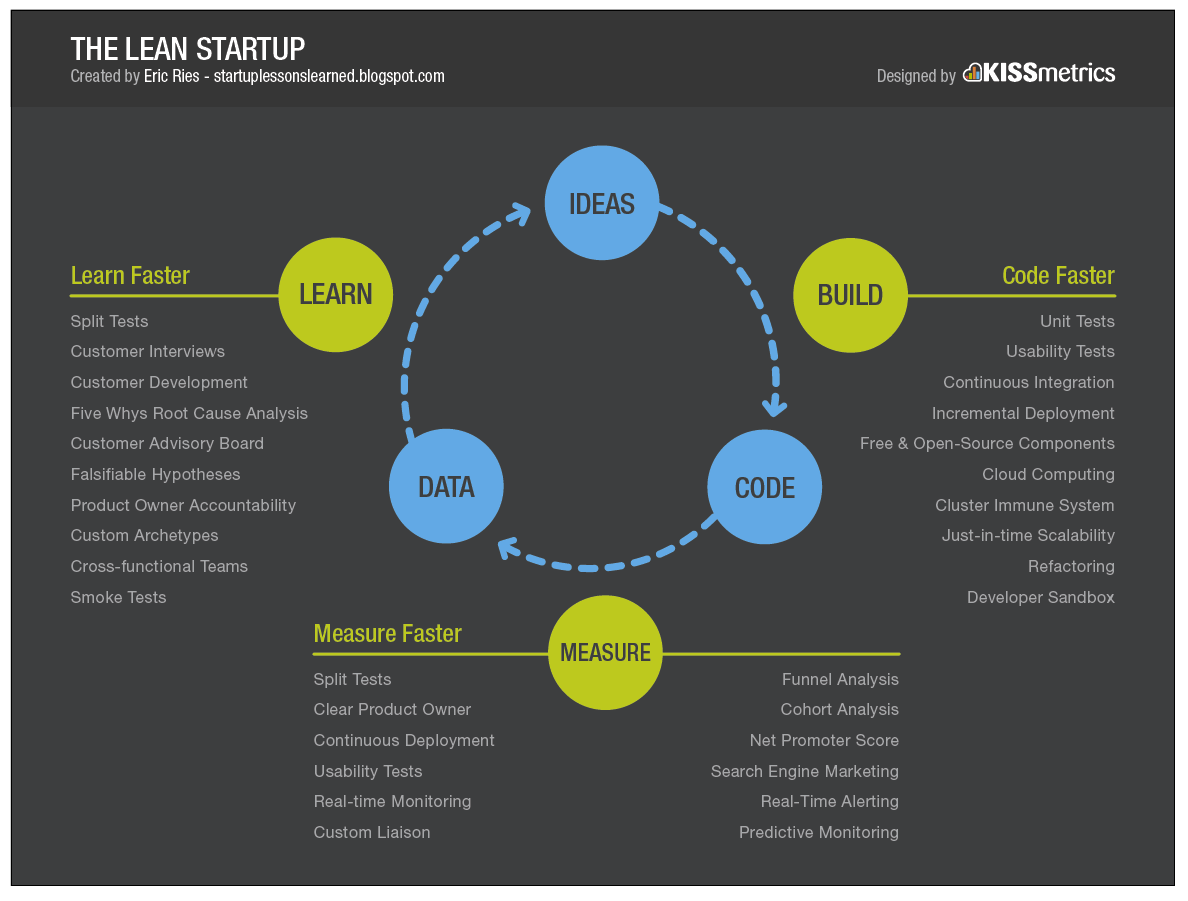
\includegraphics[height=7.5cm]{lean-flow}
\caption{Lean process model}
\end{figure}

\section{Process Models}

Both methodologies can utilize multiple process models that fit or can be adapted to adhere to their principles. Very common models are SCRUM for agile and KANBAN for lean.

\subsection{SCRUM}
SCRUM is an agile process model that focuses on having a potentially shippable product after each iteration called sprints. Each sprint normally lasts for around two weeks. The features or tasks that are worked on are taken from the backlog. The backlog is populated by user stories that have been collected from the client or product owner. They are use cases for potential features for the product

\begin{figure}[h]
\centering
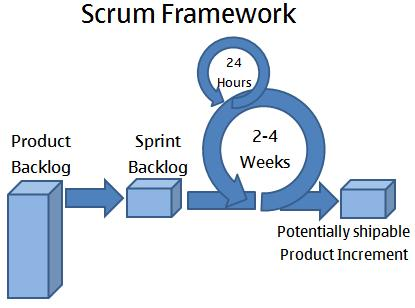
\includegraphics[height=4cm]{scrum-framework}
\caption{SCRUM process model}
\end{figure}

The SCRUM workflow begins with a planning stage for the sprint. The goal of the planning stage to to select and delegate the user stories to be completed this sprint. During this planning stage you select and evaluate the difficulty of user stories to be completed during the coming sprint. Then the daily scrum is used to say what each team member will work in the next 24 hours to achieve this goal. This is repeated until the end of the sprint. After a sprint you would have a potentially shippable product and there is a review and reflection process as well.

\subsection{Extreme Programming: XP}

Extreme programming (XP) was one of the first agile methodologies. It was designed to solve the problems of heavier, more formal methodologies and be more flexible and efficient as explained by Kent Beck, XP is a lightweight methodology for small-to-medium-sized teams developing software in the face of vague or rapidly changing requirements. [2]. XP is similar to scrum in the fact that it emphasizes frequent releases and shorter development cycles. Along with advocating pair programming, code review and unit testing on all code. The basic principles of XP are [2]:
\begin{itemize}
\item Rapid feedback
\item Assume simplicity
\item Incremental change
\item Embracing change
\item Quality work
\end{itemize}

\begin{figure}[h]
\centering

\includegraphics[height=7cm]{xp-flow}
\caption{XP process model}
\end{figure}

XP is highly flexible and can easily manage in an environment of rapidly changing requirements. It is simple and easily understood and can be implemented with any team that is familiar with agile methods and manifesto. It relies heavily on pair programming and automated unit testing.